\documentclass[article,12pt,english, a4paper, oneside, onecolumn, openany]{memoir}
\usepackage{fix-cm,fixltx2e}
\usepackage{babel}  % babel: Hyphenation patterns and language specific strings
\usepackage{varioref}
\usepackage[colorlinks,linkcolor=black,urlcolor=black,citecolor=black]{hyperref}
\usepackage[latin1]{inputenc}
\usepackage{graphicx}
\usepackage{listings}
\usepackage[square,numbers]{natbib}
\usepackage{url}
\usepackage{pslatex}
\usepackage{pdfpages}
\usepackage{placeins} % gives me FloatBarrier
%Forhindrer floats i at flyde ind i n�ste afsnit
\let\oldsection=\section % gemmer den gamle definition
\renewcommand\section{\FloatBarrier\oldsection}

\makeatletter
\renewcommand\fps@figure{htbp} % Force figure placement
\renewcommand\fps@table{htbp}
\makeatother

% setup captions
\hangcaption
\changecaptionwidth
\captionwidth{9cm}

\usepackage[margin=2.5cm]{geometry}
\linespread{1.166667}

\pagestyle{plain}
\title{Final Assignment\\\textbf{Software Architcture Analysis Report}}
\author{S�ren B. Vrist\\\url{sbvr@itu.dk}}
\begin{document}
\frontmatter
\maketitle
\tableofcontents
\newpage
\mainmatter
\chapter{Introduction}
This report will do an architechture analysis of the JCommSy software as
provided by \url{http://www.commsy.net}. The software provides a collabrative
community system for project work. 
\begin{itemize}
  \item How the system looks like(4+1 view)
  \item introduction of scope
\end{itemize}

\chapter{Theoretical foundation}
Papers:
\begin{itemize}
  \item \citep{4plus1}
  \item \citep{gqm}
  \item \citep{gqm84}
  \item \citep{docarc}
  \item \citep{ddd}
  \item \citep{slides1}
\end{itemize}
\ldots

\chapter{Intended architechture}
This section will outline the intended - or the expected if you want -
architechture of JCommSy. \\

Along with the software an image is provided as
architechtural reference. This image can be seen in figure \ref{fig:intarch} and
the following assumptions will be based on reasoning about this image and the
software.

Notice the following observations about figure \ref{fig:intarch}.
\begin{itemize}
  \item 5 horizontal layers
  \item a Cross cutting utility slice available for all layers
  \item No finegrained illustrations of vertical slices, subsystems or interface
    interactions
\end{itemize}

It is a bit backward to describe a design ``backwards'' Ie. based on existing
code and software. On one hand, if a design was part of the development process,
this would be a digging operation, trying to guess what that design is. On the
other hand if a design was not a conscious part of the software the code
``dictates'' the design in an autonomous way. The latter is not a real possibility
as described by e.g. \citep[page 70, Chapter 2.4.1]{docarc}.

Nevertheless, to have something to base this analysis on, I will set down some
``guesses'' as assumptions on the software. A way to help get a 360 feel of the
an architecture as well as illustrate different aspects of the architecture is
views\citep[Chap P.4 page 13]{docarc} and a common way to do this is the 4+1 view of
\citep{4plus1}. The four parts is Logical View, Implementation View, Process
View and Deployment View. The ``+1'' is an overlapping Use-Case View. The
reasoning behind each of these views is that each of
these views is for different stakeholders of the software and thereby preventing
misunderstandings and overly complex ``all-in-one'' diagrams \citep{4plus1}.
Other sets of views have been proposed, for example ``Functional, Static,
Distribution and Dynamic views'' by \citep{carola}. In the following the views
from \citep{4plus1} are described and some of the concepts are applied to JCommSy code.

\section{Logical View}
The logical view should show the main building blocks of the system. The
recievers of this view description is architechts and developers and should
provide an overview of the main components and their responisbilites
\citep{4plus1}. A standard way to do this is class diagrams or class categories
as described by \citep{booch}.\\

With regards to JCommSy a reasonable - albeit high-level - image of this view
could be the provided illustration as seen in \ref{fig:intarch}.

\section{Implementation View}
Created for the developers and any configuration management. This view should
give an outline of the modules, and which packages they come in. With this in
hand a developer should be able to start develop the software.

In the case of JCommSy I am a bit hindered by not knowing what the software does
and how, but by browsing the source code I would imagine you would produce
diagrams that shows subsystems like for example. ``Appointment subsystem'' as
illustrated by the code snippet in listing \ref{listing:appointment} from
CommsyServlet.java.



\chapter{Analysis}
\begin{itemize}
  \item Metrics
  \item Oberservations
\end{itemize}

\chapter{Refactoring}
\begin{itemize}
  \item identify problems (>2)
  \item Suggest actions
  \item Argue with business constraints
  \item Refactoring plan (1-2)
\end{itemize}

\chapter{Conclusion}
\ldots

\backmatter
\listoftables
%\listoffigures

\bibliography{biblio}
\bibliographystyle{alphaurl}
\clearpage
\appendix
\chapter{Listings}
\lstset{
language=java,
basicstyle=\tiny,
numbers=left,
}

\begin{lstlisting}[caption={Extract from CommsyServlect.java},label=listing:appointment,firstnumber=235]
  if (parameter.getModuleString().equals(MODULE_APPOINTMENT)
  || parameter.getModuleString().equals(MODULE_DISCUSSION)
  || parameter.getModuleString().equals(MODULE_ANNOUNCEMENT)
  || parameter.getModuleString().equals(MODULE_GROUP)
  || parameter.getModuleString().equals(MODULE_MATERIAL)
  || parameter.getModuleString().equals(MODULE_TODO)
  || parameter.getModuleString().equals(MODULE_TOPIC)
  || parameter.getModuleString().equals(MODULE_USER)
  || parameter.getModuleString().equals(MODULE_RSS)) {
  getServletContext().getNamedDispatcher(LogicServlet.class.getSimpleName()).forward(request, response);
\end{lstlisting}

\chapter{Figures}
\section{Architechture image}
\begin{figure}
  \centering
  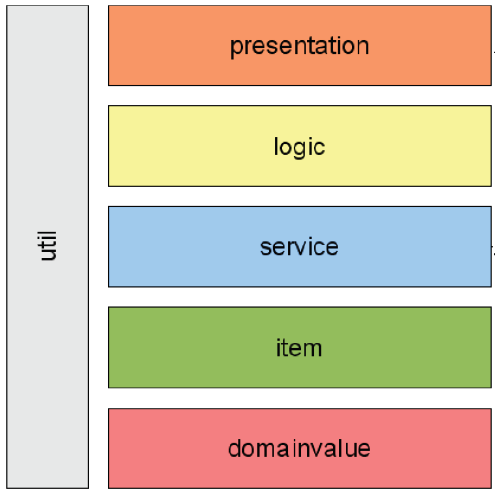
\includegraphics[width=11cm]{arch}
  \caption{The given overview of JCommSy architechture}\label{fig:intarch}
\end{figure}
\end{document}
